\documentclass[12pt, twoside, a4paper]{article}

%pdfTeX
% \usepackage[utf8]{inputenc}
% \usepackage[T1]{fontenc}

\usepackage[margin=1truein]{geometry}

% \usepackage{palatino}
% \usepackage{charter}


\usepackage{amsmath}
\usepackage{amssymb}
\usepackage{graphicx}
\usepackage[figurename=Slika,labelfont=bf]{caption}
\usepackage{tabularx}
\usepackage{mathtools}
\usepackage{pdflscape}
\usepackage{rotating}
\usepackage{enumitem}

\usepackage[dvipsnames]{xcolor}

\definecolor{darkblue}{rgb}{0, 0, 0.4}
\usepackage[
  colorlinks = true,
  urlcolor = darkblue,
  linkcolor = black
]{hyperref}

\usepackage{qrcode}
\usepackage{svg}
\usepackage{wrapfig}

\usepackage{totcount}
\newtotcounter{zadaci}
\setcounter{zadaci}{0}

\input serbian


\DeclareGraphicsRule{*}{mps}{*}{}

\renewcommand*\contentsname{Sadr{\zv}aj}

\usepackage{titlesec}
\newcommand{\sectionbreak}{\clearpage
  \vskip 0.75in plus 0.25in minus 0.25in\relax}
%\newcommand{\subsectionbreak}{\clearpage}

\definecolor{ZXink}{rgb}{0.25, 0.25, 0.25}
\definecolor{ZXpaper}{rgb}{0, 1, 1}
%\def\aspect{.618034}
\def\aspect{1}

\def\bitrow#1{{\hbox{\count0=7\relax\count1=#1\relax
\vrule width 0pt height \dimen0 depth 0pt\relax
\loop
\ifnum\count1<128\relax
\kern \aspect\dimen0\relax
%\kern .707101\dimen0\relax
%{\color{ZXpaper}\vrule width .70711\dimen0 height \dimen0 depth 0pt}\relax
\else
%{\color{ZXink}\vrule width .707101\dimen0 height \dimen0 depth 0pt}\relax
{\color{ZXink}\vrule width \aspect\dimen0 height \dimen0 depth 0pt}\relax
\advance\count1 by -128\relax
\fi
\advance\count1 by \count1\relax
\advance\count0 by -1\relax
\unless\ifnum\count0<0\repeat}}}

\newbox\zxbox
\def\bitbox#1#2#3#4#5#6#7#8{{\setbox\zxbox\hbox{0}%
\dimen0=\ht\zxbox \divide\dimen0 by 6\relax
\lower\dimen0\vbox{\offinterlineskip
\bitrow{#1}\bitrow{#2}\bitrow{#3}\bitrow{#4}\bitrow{#5}\bitrow{#6}\bitrow{#7}\bitrow{#8}}}}
\def\ZXL{\bitbox{0}{64}{64}{64}{64}{64}{126}{0}}
\def\ZXE{\bitbox{0}{126}{64}{124}{64}{64}{126}{0}}
\def\ZXT{\bitbox{0}{254}{16}{16}{16}{16}{16}{0}}
\def\ZXspace{\bitbox00000000}
\def\ZXr{\bitbox{0}{0}{28}{32}{32}{32}{32}{0}}
\def\ZXdollar{\bitbox{0}{8}{62}{40}{62}{10}{62}{8}}
\def\ZXeq{\bitbox000{62}0{62}00}
\def\ZXquote{\bitbox0{36}{36}00000}
\def\ZXzero{\bitbox0{60}{70}{74}{82}{98}{60}0}
\def\ZXone{\bitbox0{24}{40}888{62}0}
\def\ZXZ{\bitbox0{126}48{16}{32}{126}0}
\def\ZXX{\bitbox0{66}{36}{24}{24}{36}{66}0}
\def\ZXB{\bitbox0{124}{66}{124}{66}{66}{124}0}
\def\ZXA{\bitbox0{60}{66}{66}{126}{66}{66}0}
\def\ZXS{\bitbox0{60}{64}{60}2{66}{60}0}
\def\ZXI{\bitbox0{62}8888{62}0}
\def\ZXC{\bitbox0{60}{66}{64}{64}{66}{60}0}

\def\BASIC{\leavevmode\ZXB\ZXA\ZXS\ZXI\ZXC\relax}
\def\ZXBASIC{\leavevmode\ZXZ\ZXX\ZXspace\ZXB\ZXA\ZXS\ZXI\ZXC\relax}
\def\LETr#1{\ZXL\ZXE\ZXT\ZXspace\ZXr\ZXdollar\ZXeq\ZXquote#1\ZXquote\relax}

\newdimen\zxpx \zxpx=0.25mm
\newdimen\zxscreen \zxscreen=320\zxpx


\font\eightss=cmssq8
\font\eightssi=cmssqi8

\def\K{\mathop{\vcenter{\hbox{\rm\huge K}}}\limits}
\def\n{n}
\def\Ki{\K_{\n=1}}
\def\Kinf#1#2{\Ki^\infty\displaystyle{\frac{#1}{#2}}}

\def\mul{{\cdot}}
\def\navod#1{\relax,\kern-0.06667em,\relax#1\relax``\relax}

\def\logten{\log_{10}}
\def\logtwo{\log_2}
\def\loga{\log_a}
\def\logb{\log_b}
\def\puta{\times}
\def\comma{{,}}
\let\dotacc=\.
\def\.{{,}}
\def\e{{\bf e}}
%\def\naplog{\mathop{\mathop{\rm Log}\limits^{\rm Nap}}\nolimits}
\def\naplog{\mathop{\rm NapLog}\nolimits}
\def\QED{\ensuremath{\qquad\square}}
\def\th{t_{1/2}}
\def\um#1{\,{\rm#1}}
\newdimen\mm \mm=1truemm
\def\cis{\mathbin{\rm cis}}

\def\marg#1{\raise1pt\hbox{\colorbox{Aquamarine}{\color{white}\hbox to 1em{\hss\eightss#1\/\hss}}}}
\def\ram#1{\,\fcolorbox{black}{white}{$\,\displaystyle{\mathstrut #1}\,$}\,}
\def\okvir#1{\fcolorbox{black}{Goldenrod}{$\,\displaystyle{\mathstrut #1}\,$}}
\def\sledi{{\quad\Rightarrow\quad}}

\newcount\exno \exno=0
\def\zabox#1{\leavevmode\hbox to 5.2em{{\bf #1}\hfill}}
\def\zadatak{\global\advance\exno by 1\relax
  \addtocounter{zadaci}{1}
  \par\noindent\leavevmode
  \llap{$\vartriangleright\>$}%
  \hbox to 0pt{\kern\textwidth\kern2em{\marg{\the\exno}}\hss}%
  \zabox{Zadatak:}}
\def\resenje{\par\medskip\noindent\leavevmode
  \llap{$\blacktriangleright\>$}\zabox{Re{\sv}e{\nj}e:}}
\def\dodatak{\par\medskip\noindent\leavevmode
\llap{$\vcenter{\hbox{$\scriptstyle\bigstar$}}\>$}\zabox{Dodatak:}}

%\def\dodatak{\par\medskip\noindent\zabox{Dodatak:}}
\newcommand{\rsinfty}{{\,\widetilde{\!\infty\!}\,}}

\def\GitHub{https://github.com/Nasumica/LukaMaturski/}
\def\GitHubMain{\GitHub blob/main/}
\def\GitHubRaw{\GitHub raw/refs/heads/main/}

\parindent=24pt

\begin{document}

\input titlepage

\tableofcontents


\section{Uvod}

Ovaj rad se bavi {\sl logaritamskom funkcijom}, jednom od najva{\zv}nijih funkcija u matematici.
Zbog svoje va{\zv}nosti, zajedno sa eksponencijalnom,
trigonometrijskim i {\nj}ima inverznim funkcijama, spada u grupu {\sl elementarnih funkcija}. 
Opisane su {\nj}ene osobine i dati su primeri {\nj}ene upotrebe,
kao i zadaci sa re{\sv}e{\nj}ima (ukupno \the\numexpr\totvalue{zadaci}).



\subsection{Definicija logaritma}

Ako je
$$
x=b^y
$$
onda se mo{\zv}e pisati
\begin{equation}
\okvir{y=\log_b x},
\end{equation}
gde je $b$ {\sl osnova\/} ({\sl baza\/}) logaritma, a $x$ {\sl argument}.
(Izgovara se \navod{$y$ je jednako logaritam od $x$ za osnovu $b$}
ili kra{\cc}e \navod{$y$ je logaritam $b$ od $x$}.)
Tako{\dj}e va{\zv}i
$
b=x^{1/y}=\sqrt[y]x.
$

Sama re{\cv} {\sl logaritam\/} poti{\cv}e od gr{\cv}kih re{\cv}i 
$\lambda\acute o\gamma o\varsigma$~({\sl logos\/}) i 
$\acute\alpha\rho\iota\theta\mu\acute o\varsigma$~({\sl aritmos\/}), 
sa zna\-{\cv}e\-{\nj}em \navod{broj kojim se ra{\cv}una}.


\subsection{Grafik funkcije}

\newcounter{figno}
\def\newpic#1{\stepcounter{figno}%
  \hbox{{\bf Slika \thefigno:\/~}#1}}
\def\slika#1#2{\stepcounter{figno}\displaylines{
  \hbox{#1}\cr\hbox{{\bf Slika \thefigno:\/~}#2}}}


Funkcija je u skupu realnih brojeva ${\mathbb R}$ definisana za $x>0$ i $b>0\land b\ne1$.
Funkcija je {\sl monotona\/}: za $b>1$ funkcija je {\sl rastu{\cc}a}, dok je za $b<1$ funkcija {\sl opadaju{\cc}a}.
Zbog toga va{\zv}i {\sl bijekcija\/}: $\logb x=\logb y \Leftrightarrow x=y$.
Funkcija ima jednu {\sl nulu}, uvek za $x=1$.
$$
\slika{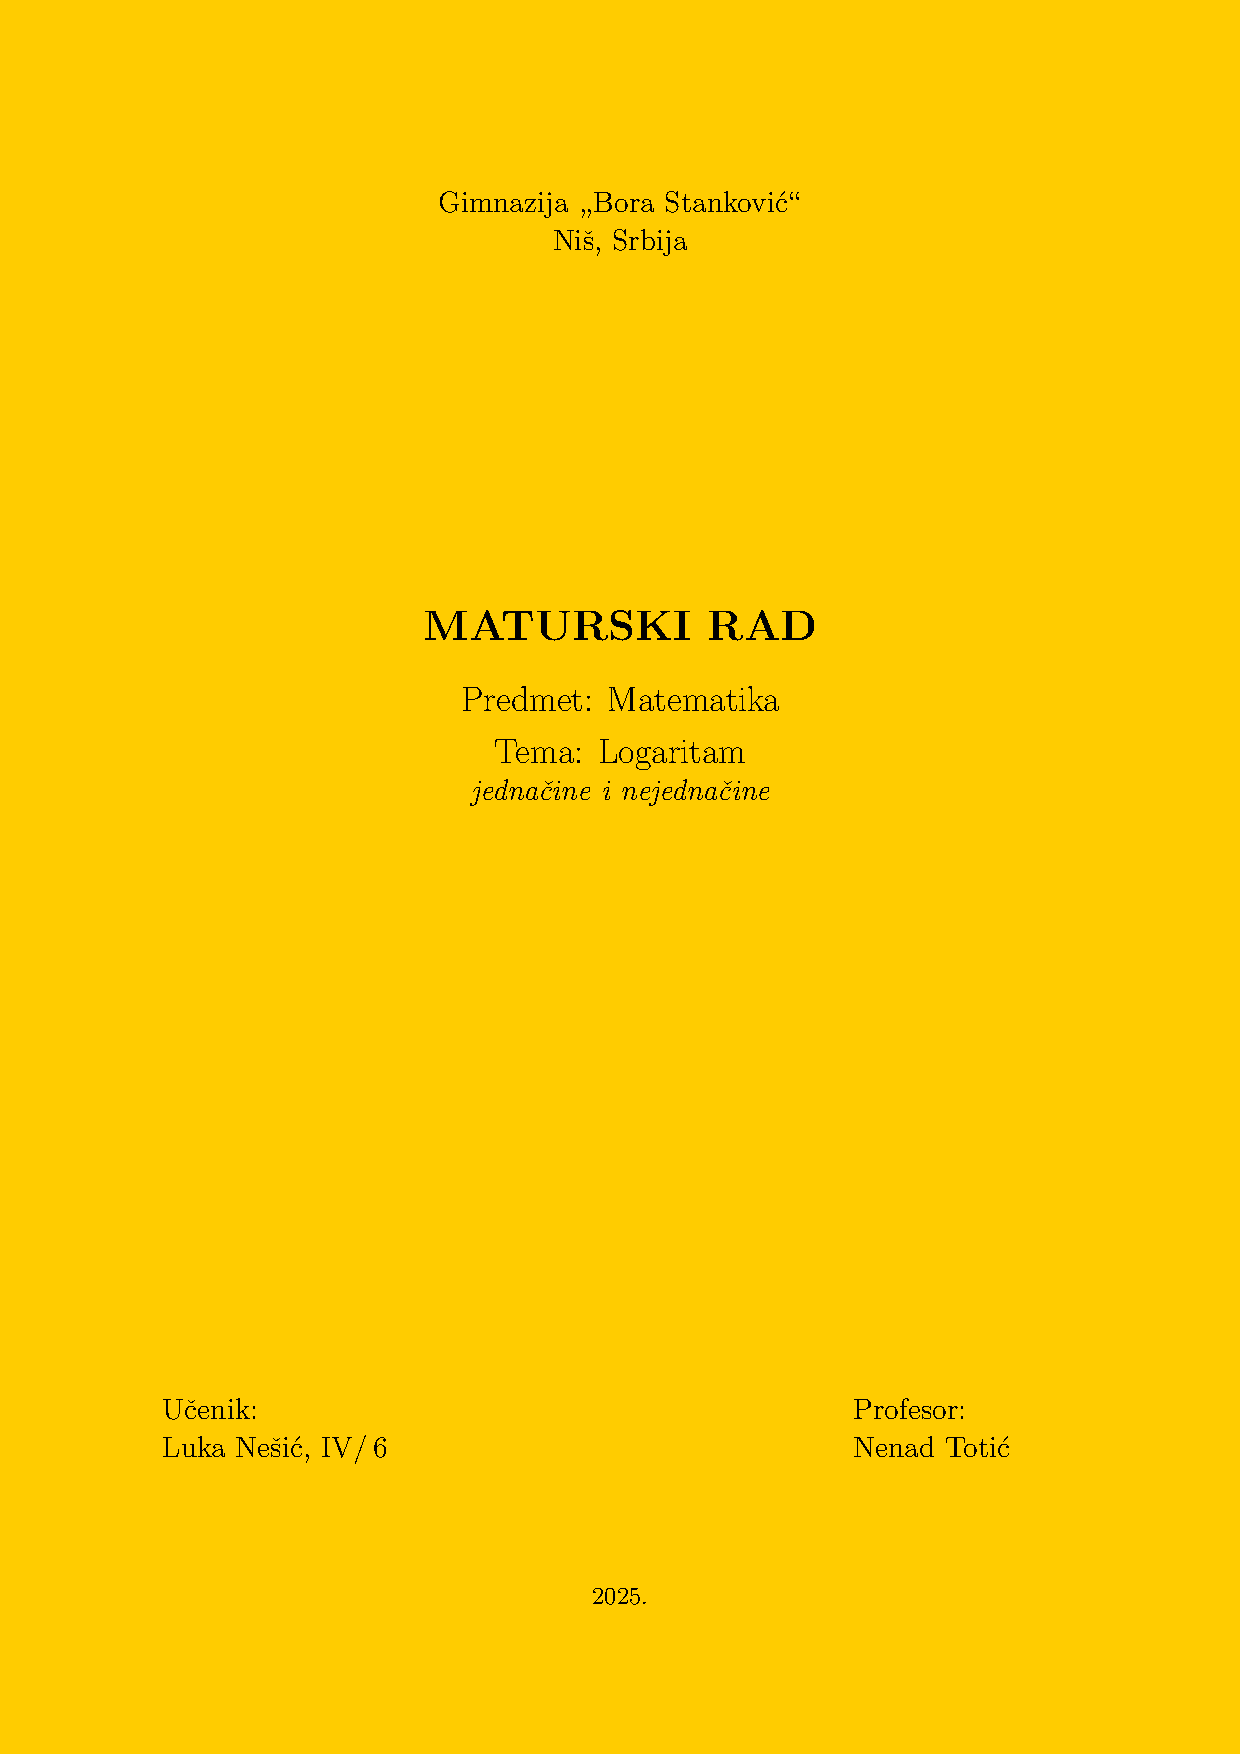
\includegraphics[]{log.1}}{Grafik logaritamske funkcije $y=\logb x$.}
$$

\subsection{Antilogaritam}

\def\antilog{\mathop{\rm anti\,log}\nolimits}
Inverzna funkcija logaritmu
je obi{\cv}no stepenova{\nj}e osnove logaritma argumentom i zove se {\sl antilogaritam}
\begin{equation}
\okvir{\antilog_bx = \logb^{-1}x =  b^x}.
\end{equation}
Iz same definicije va{\zv}i
\begin{equation}
\okvir{\log_b(\antilog_b x)=\antilog_b(\log_b x)=x}.
\end{equation}



\section{Jednakosti}

Za logaritamsku funkciju va{\zv}e razne {\sl jednakosti\/} koje se koriste za 
upro{\sv}{\cc}iva{\nj}e i pri\-la\-go\-{\dj}a\-va\-{\nj}e izraza prilikom re{\sv}ava{\nj}a
problema i zadataka.

\subsection{Logaritam stepena osnove}

Po samoj definiciji logaritma, ako je $x=b^a$, onda je
\begin{equation}
\okvir{\logb b^a=a}.
\label{eq:powb}
\end{equation}
Ako stavimo da je $1=b^0$, odnosno, $b=b^1$, dobijamo da je
\begin{equation}
\okvir{\logb 1=0}\qquad\text{i}\qquad\okvir{\logb b=1}.
\end{equation}
Tako{\dj}e je bitna jednakost
\begin{equation}
\okvir{b^{\logb x}=x}
\end{equation}
koja proizilazi iz same definicije logaritma i antilogaritma.

\subsection{Logaritam proizvoda}

Ako je
$$
u=\logb x\land v=\log_b y \sledi x=b^u\land y=b^v,
$$
onda je, zbog jednakosti \eqref{eq:powb}
$$
x\cdot y=b^ub^v=b^{u+v}\sledi \logb(x\cdot y)=\logb b^{u+v}=u+v.
$$
Odavde je
\begin{equation}
\okvir{\logb(x\cdot y)=\logb x+\logb y}.
\label{eq:lnmul}
\end{equation}

Iz ove jednakosti se mo{\zv}e izvesti formula za logaritam faktorujela broja. Ako je
$$
n!=\prod_{k=1}^n k\sledi \log(n!)=\sum_{k=1}^n\log k.
$$
(Zanim{\lj}ivo je da je $\log(1\cdot2\cdot3)=\log(1+2+3)=\log1+\log2+\log3$.)


\subsection{Logaritam koli{\cv}nika}

Sli{\cv}no logaritmu proizvoda, 
ako je
$$
u=\logb x\land v=\log_b y \sledi x=b^u\land y=b^v,
$$
onda je, zbog jednakosti \eqref{eq:powb}
$$
x/ y=b^ub^{-v}=b^{u-v}\sledi \logb(x/y)=\logb b^{u-v}=u-v.
$$
Odavde je
\begin{equation}
\okvir{\logb(x/ y)=\logb x-\logb y}.
\label{eq:lndiv}
\end{equation}
Iz ove jednakosti sledi
\begin{equation}
\okvir{\logb(1/x)=-\logb x}.
\label{eq:recip}
\end{equation}

\subsection{Logaritam stepena broja}

Ako je
$$
y=x^n=\underbrace{x\cdot x\cdots x}_{\text{$\mathstrut n$ puta}},
$$
onda, iz jednakosti za logaritam proizvoda \eqref{eq:lnmul}, sledi da je
$$
\logb y=\logb (\underbrace{\mathstrut x\cdot x\cdots x}_{\text{$n$ puta}})
=\underbrace{\mathstrut \logb x+\logb x+\cdots+\logb x}_{\text{$n$ puta}}
=n\logb x,
$$
odakle je
\begin{equation}
\okvir{\logb x^n=n\logb x}.
\label{eq:bpow}
\end{equation}
Iz ove jednakosti sledi jednakost
\begin{equation}
\okvir{\logb\sqrt[n] x=\frac1n\logb x},
\label{eq:lnroot}
\end{equation}
kao i jednakost
\begin{equation}
\okvir{x^y=b^{y\logb x}}.
\label{eq:power}
\end{equation}


\subsection{Promena osnove logaritma}

Ako je
$$
y = \loga x\sledi x = a^y,
$$
onda je 
$$
\logb x=\logb a^y=y\logb a=\loga x\cdot\logb a.
$$
Odavde je
\begin{equation}
\okvir{\loga x=\frac{\logb x}{\logb a}}.
\label{eq:chgbase}
\end{equation}
Iz ove jednakosti, ako stavimo da je $x=b$, se dobija i jednakost
\begin{equation}
\okvir{\loga b\cdot\logb a = 1}.
\end{equation}
Iz jednakosti \eqref{eq:powb} i \eqref{eq:chgbase}, ako stavimo da je $a=b^n$, sledi jednakost
\begin{equation}
\okvir{\log_{b^n}x = \frac1n \logb x}.
\label{eq:powbase}
\end{equation}
Odavde, ako stavimo da je $n=-1$, sledi
\begin{equation}
\okvir{\log_{1/b}x = -\logb x},
\end{equation}
a uzev{\sv}i u obzir i jednakost \eqref{eq:recip} dobija se
\begin{equation}
\okvir{\log_{1/b}x = \logb(1/x)}.
\end{equation}

\bigskip

\font\manfnt=manfnt scaled 1200 % 1.2 * sqrt(1.2) * 1000
\def\dbend{{\manfnt\char126\relax}}
\def\danger#1\par{\begingroup\hangindent=\parindent 
\hangafter=-2 \noindent\leavevmode
\smash{\hbox to 0pt{\kern-\hangindent\lower1.2pt\hbox{\dbend}\hss}}%
#1\par\endgroup}


\danger\label{danger}%\textbf{Napomena:\/}
Treba biti oprezan kod kori{\sv}{\cc}e{\nj}a svih ovih jednakosti, naro{\cv}ito kod ste\-pe\-no\-va{\nj}a, 
i~uvek treba proveriti interval u kome se ra{\cv}una.
Na primer, iz jed\-na\-ko\-sti~\eqref{eq:bpow}, sledi $\log x^2=2\log x$, {\sv}to je ispravno za $x>0$,
a~ina{\cv}e, $\log x^2=2\log|x|$, za bilo koje $x\ne0$. 
Ili, iz jednakosti~\eqref{eq:bpow} i~\eqref{eq:powbase}, $\log_{b^2}x^2 = \log_{|b|}|x|$,
i sli{\cv}ne varijacije.

\section{Naj{\cv}e{\sv}{\cc}e logaritamske osnove}

\subsection{Osnova 10}

U ini{\zv}e{\nj}erstvu se naj{\cv}e{\sv}{\cc}e koristi osnova logaritma 10,
zove se {\sl dekadni\/} ili {\sl zajedni{\cv}ki\/} logaritam, i pi{\sv}e se
$$
y=\logten x
$$
ili, skra{\cc}eno,
$$
y=\lg x.
$$
Ponekad se mo{\zv}e videti i samo
$$
y=\log x,
$$
bez navo{\dj}e{\nj}a osnove, ali treba obratiti pa{\zv}{\nj}u na kontekst.
Ako je neki in{\zv}e{\nj}erski tekst u pita{\nj}u, najverovatnije se misli na osnovu 10.

Dekadni logaritam je pogodan i kada se koristi, takozvani {\sl nau{\cv}ni\/} ili {\sl in{\zv}e{\nj}erski\/}
zapis broja.
Na primer, {\sl Plankova konstanta\/} (Max Planck) iznosi
$$
h=6\.62607015\puta 10^{-34}
$$
koja ima dekadni logatiram
$$
\logten h=\logten(6\.62607015) - 34.
$$

U fizici se za mere{\nj}e nivoa signala ili zvuka koristi jedinica {\sl be\/l}~(B), ali je {\cv}e{\sv}{\cc}e
u prakti{\cv}noj upotrebi 10 puta ma{\nj}a jedinica {\sl decibel\/}~(dB), odnosno, $1\um{B}=10\um{dB}$. \
Nivo \hbox{sig\-na\-la} $L$, koji zavisi
od odnosa izmerene snage $P$ i refrentne snage $P_0$, izra{\zv}en u deci\-belima iznosi
$$
L=10\logten\left(\frac{P}{P_0}\right)\um{dB}.
$$
Kako se u akustici uzima da je referentna snaga $P_0=10^{-12}\um W$, moglo bi se pisati
da je nivo zvuka u decibelima
$$
L=10\logten(P)-120.
$$

Normalan govor je oko $50\um{dB}$, 
zvuk motora mlaznog aviona pri poleta{\nj}u je $150\um{dB}$, 
%raketa Saturn~V oko $220\um{dB}$,
a smrtonosan je zvuk od $240\um{dB}$ i vi{\sv}e.
Zvu{\cv}ni top {\sf Genasys LRAD} ima nivo zvuka od oko $160\um{dB}$,
{\sv}to zna{\cv}i da je $10^{11}$ puta mo{\cc}niji od govora.
%Naravno, treba uzeti u obzir da nivo opada sa kvadratom rastoja{\nj}a.

Sli{\cv}na formula se koristi i za odre{\dj}iva{\nj}e ja{\cv}ine zem{\lj}otresa, ili pH vrednosti.
% $M=\logten I$, gde je $M$ magnituda po {\sl Rihterovoj skali}, a $I$ intenzitet.

\subsection{Osnova 2}

\def\lb{\mathop{\rm lb}}
\def\bits{{\it bits}}
\def\mant{{\it mantisa}}%
\def\expo{{\it eksponent}}%
\def\znak{{\it znak}}%

U informatici se {\cv}esto koristi logaritam sa osnovom 2, koji se zove {\sl binarni\/} logaritam,
i pi{\sv}e se
$$
y=\logtwo x
$$
ili, skra{\cc}eno,
$$
y=\lb x.
$$
Koristi se u kombinatorici, kao i u odre{\dj}iva{\nj}u {\sl koli{\cv}ine informacija},
odnosno, potrebnog broja bitova me\-mo\-ri\-je za sme{\sv}ta{\nj}e nekog podatka.
Ako se zna da {\cc}e u me\-mo\-ri\-ju biti upisivani celi brojevi od 0 do $n$, onda je potrebno rezevisati
$$
\bits = \lfloor\logtwo(n)\rfloor+1
$$
bitova memorije, gde $\lfloor x\rfloor$ predstav{\lj}a {\sl najve{\cc}i ceo broj koji je ma{\nj}i ili jednak} $x$
(izgovara se \navod{najve{\cc}e celo od $x$}). 
Na primer, ako {\cc}e u odre{\dj}enoj memoriji najve{\cc}i 
broj biti milion, onda je za to potrebno rezevisati
$$
\bits=\lfloor\logtwo(1\,000\,000)\rfloor+1=\lfloor 19\.9315685693\rfloor+1 = 19+1=20
$$
bitova memorije. Najve{\cc}i broj koji mo{\zv}e stati u ovih rezervisanih 20 bitova memorije je binarni broj koji ima 20 jedinica
i iznosi 
$$
(1111\,1111\,1111\,1111\,1111)_2=
2^{20}-1=1\,048\,575.
$$

Kako su i realni brojevi u memoriji predstav{\lj}eni kao ure{\dj}eni parovi binarnih brojeva u obliku
$(\mant,\expo)$, sa zna{\cv}e{\nj}em
$$
x=\mant\puta2^\expo,
$$
binarni logaritam bi bio izra{\cv}unat kao
$$
\logtwo(x)=\logtwo(\mant)+\expo,
$$
ako je $\mant>0$, ina{\cv}e je nedefinisan.

\smallskip

Binarni logaritam se koristi i u atomskoj fizici.
Vreme {\sl poluraspada\/} $\th$ je vreme potrebno da se raspadne polovina jezgara atoma neke materije. 
Ako imamo po{\cv}etan broj jezgara $N_0$ i broj jezgara $N_t$ nakon vremena $t$, njihov odnsos
se mo{\zv}e pred\-sta\-vi\-ti formulom
\begin{equation}
\label{eq:halftime}
\frac{N_0}{N_t}=2^{t/\th}\sledi \frac{t}{\th}=\logtwo\left( \frac{N_0}{N_t} \right).
\end{equation}
Ova formula se koristi i za odre{\dj}iva{\nj}e starosti stena ili fosila.


%\clearpage

\subsection{Osnova \e}

Ovu logaritamsku osnovu je otkrio Jakob Bernuli (Jacob Bernoulli) kada je
prou{\cv}avao {\sl slo{\zv}enu kamatu\/} i dokazao da {\sl kontinualna\/} slo{\zv}ena kamata
te{\zv}i konstanti
$$
\e=\lim_{n\to\infty}\left(1+\frac1n\right)^{\!n}\!,
$$
ali je Ojler (Leonhard Euler)
odredio {\nj}enu vrednosti i dao joj ime.
Logaritam za ovu osnovu se zove {\sl prirodni\/} logaritam ({\sl logarithmus naturalis\/})
i pi{\sv}e se
$$
\ln x=\log_\e x.
$$

\def\ep{\hphantom{!}}
\def\rf#1!{\frac1{\hphantom{!}#1!}}
Antilogaritam je $\e^x$, koji se kao funkicja pi{\sv}e $\exp(x)$, i zove se
{\sl eksponencijalna funkcija}. Ova funkcija je poznata po tome {\sv}to je to 
jedina funkcija {\cv}iji je izvod jednak samoj funkciji. Brojna vrednost se mo{\zv}e
izra{\cv}unati formulom
\begin{equation}
\label{eq:exp}
\okvir{\e^x=\exp(x)=\sum_{n=0}^\infty\frac{x^n}{n!}}.
\end{equation}
Ako stavimo da je $x=1$,
brojna vrednost osnove prirodnog logaritma $\e$ se mo{\zv}e odrediti
\begin{equation}
\label{eq:e}
\begin{aligned}
\e
&=\rf0!+\rf1!+\rf2!+\rf3!+\rf4!+\rf5!+\cdots\\
&=2\.
7182818284\,
5904523536\,
0287471352\,
6624977572\,\ldots
\end{aligned}
\end{equation}
sa {\zv}e{\lj}enom ta{\cv}no{\sv}{\cc}u.


\section{Brojna vrednost}

\subsection{Formula}

Brojna vrednost prirodnog logaritma mo{\zv}e biti izra{\cv}unata pomo{\cc}u formule
\begin{equation}
\okvir{
\ln x
%&=2\mathop{\rm arctanh}\frac{x-1}{x+1}\\
=\sum_{n=0}^\infty\frac{2}{2n+1}\left(\frac{x-1}{x+1}\right)^{\!2n+1}
}
\label{eq:lnred}
\end{equation}
do {\zv}e{\lj}ene ta{\cv}nosti.
Postupak kojim se ra{\cv}una $y=\ln x$ sa ta{\cv}no{\sv}{\cc}u $\varepsilon$
izgleda ovako:
\def\asg{\leftarrow}%
\begin{equation}
\label{eq:alg}
\begingroup\color{Blue}
\ram{\enspace
\begin{aligned}
&r\asg(x-1)/(x+1);\quad k\asg 1;\quad p\asg 2r;\quad q\asg r^2;\quad a\asg p;\quad y\asg a;\\
&\text{ponav{\lj}ati dok je $|a|>\varepsilon$:}\\
&\qquad k\asg k+2;\quad p\asg p\cdot q;\quad a\asg p/k;\quad y\asg y+a;
\end{aligned}
\enspace}
\endgroup
\end{equation}
(Videti zadatak \ref{sssec:ln3} na strani \pageref{sssec:ln3}.)
Ovim postupkom se mo{\zv}e izra{\cv}unati vrednost
\label{ln2}
\begin{align*}
\ln2
&=\frac{2}{1\cdot3^1}+\frac{2}{3\cdot3^3}+\frac{2}{5\cdot3^5}+\frac{2}{7\cdot3^7}+\frac{2}{9\cdot3^9}+\cdots\nonumber \\
\noalign{\smallskip}
&= 0\.
6931471805\,
5994530941\,
7232121458\,
1765680755\,
\ldots
\intertext{kao i vrednost}
\ln 10&=2\.
3025850929\,
9404568401\,
7991454684\,
3642076011\,
\ldots
\end{align*}
Ove vrednosti se koriste prilikom izra{\cv}unava{\nj}a vrednosti binarnog, odnosno, de\-kad\-nog logaritma
$$
\lb x=\logtwo x=\frac{\ln x}{\ln2},\qquad \lg x=\logten x=\frac{\ln x}{\ln 10}.
$$

\subsection{Veri{\zv}ni razlomak}

Brojna vrednost prirodnog logaritma mo{\zv}e se izra{\cv}unati i pomo{\cc}u {\sl veri{\zv}nog razlomka}
\begin{align*}
\ln(1+x)
&=\cfrac{x}{1+\cfrac{1^2x}{2-1x+\cfrac{2^2x}{3-2x+\cfrac{3^2x}{4-3x+\ddots}}}}\\
\noalign{\vskip-3pt}
&=\cfrac{x}{1+ \Kinf{\n^2x}{\n+1-\n x}}.
\end{align*}
Poput simbola koji se koriste za sumu `$\rm\Sigma$' ili proizvod `$\rm\Pi$', 
Gaus (Carl Friedrich Gauss) je smislio, verovatno, najpogodniji na{\cv}in za predstav{\lj}a{\nj}e
veri{\zv}nih (lan{\cv}anih) razlomaka,
gde simbol `K' poti{\cv}e od nema{\cv}ke re{\cv}i za {\sl prekinuti lanac\/} ({\sl Kettenbruch\/}). 
Izraz iza ovog simbola pokazuje kako izgleda {\sl op{\sv}ti {\cv}lan\/} veri{\zv}nog razlomka.

\def\ff#1/#2,{\frac{#1}{#2},}
Ako pomo{\cc}u ove formule izra{\cv}unamo prvih 11 {\sl konvergenata} $\ln2$ kao $-\ln(1-1/2)$, dobi{\cc}emo
$$
\ln2\approx\ff1/2, \ff5/8, \ff2/3, \ff131/192, \ff661/960, \ff1327/1920, \ff1163/1680, \ff148969/215040, 
\ff447047/645120, \ff44711/64512, \ff983705/1419264, \dots
$$
gde je posled{\nj}i razlomak ta{\cv}an na 5 decimala.


\subsection{Logaritamske tablice}

Prve tablice logaritama je izra{\cv}unao Neper (John Napier of Merchiston)
1614.\ godine,
koje su prakti{\cv}no sadr{\zv}ale logaritam za osnaovu $1/\e$, sa skaliranim argumentom i rezultatom,
iako sam Neper nije znao za konstantu $\e$.
Savremenim zapisom bi ovaj logaritam bio definisan kao
$$
\naplog (x) = 10^7\log_{1/\e}(x/10^7) = -10^7\ln(x/10^7).
$$

Nekoliko godina kasnije, 1617.\ i 1624, Brigs (Henry Briggs) je izra{\cv}unao
tablice de\-kad\-nih logaritama sa 14 cifara ta{\cv}nosti, koje se uz dopune i ispravke
koriste i danas pod imenom {\sl Brigsove tablice}.


\subsection{Logaritmar}

\input siber

Pre pojave digitrona, za pribli{\zv}no odre{\dj}iva{\nj}e
brojne vrednosti logaritma,
koristila se je analogna mehani{\cv}ka sprava sa nekoliko le{\nj}ira zvana {\sl logaritmar}.
$$
\slika{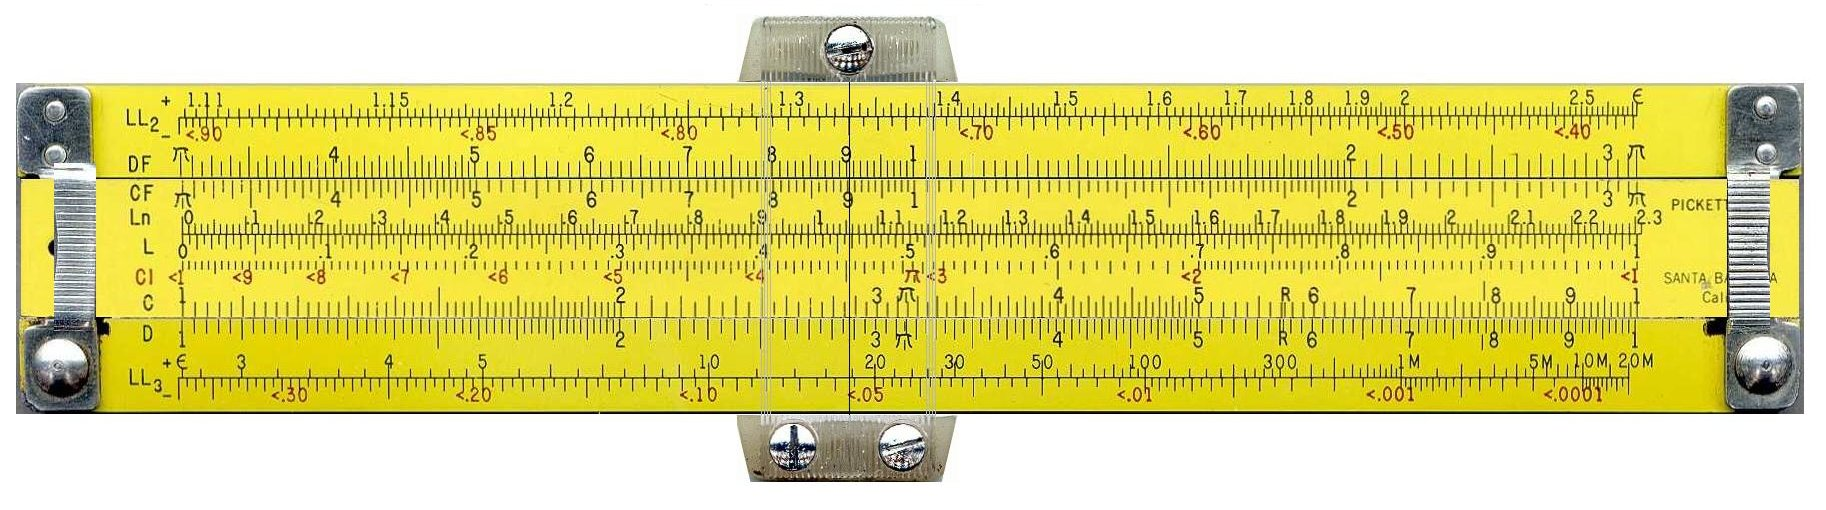
\includegraphics[width=0.90\textwidth]{siber2.jpg}}{{\Sv}iber.}
$$
Le{\nj}iri imaju podeoke sa decimalom i logaritamskom, a {\cv}esto i sa sinusnom skalom.
Jedan od le{\nj}ira je bio klizni, te otuda popularno ime {\sl{\sv}iber\/}
(od nema{\cv}kog {\sl Rechen\-schieber\/}). Koristi se jednostavno, pomera{\nj}em
kliza{\cv}a i {\cv}ita{\nj}em vrednosti sa odgovaraju{\cc}e skale.
(Videti za\-da\-tke~\ref{sssec:sibersqrt} i~\ref{sssec:siberpower}.)

Postojale su i kru{\zv}ne varijante, pa i {\dz}epne, gde je
{\dz}epni sat sa logaritmarom i kompasom  bio \navod{iPhone} XIX i prve polovine XX~veka.
$$
\slika{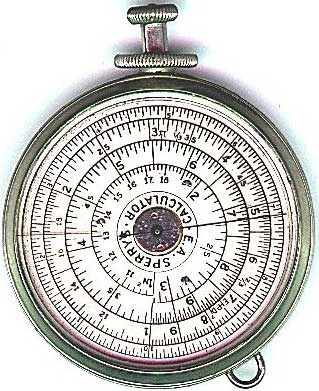
\includegraphics[width=50\mm]{sahat.jpg}}{{\Dz}epni logaritmar.}
$$

Tablice i logaritmari se i danas koriste u vojsci, kao rezerva u slu{\cv}aju otkaziva{\nj}a elektronike.
Prvi kompjuter ENIAC (Electronic Numerical Integrator And Computer)
je naprav{\lj}en 1946. godine da bi izra{\cv}unao tablice za vojsku.


\section{Jo{\sv} pone{\sv}to}

\subsection{Kompleksni logaritam}

Ako u kompleksnoj ravni imamo kompleksan broj $z\in{\mathbb C}$, 
$$
\slika{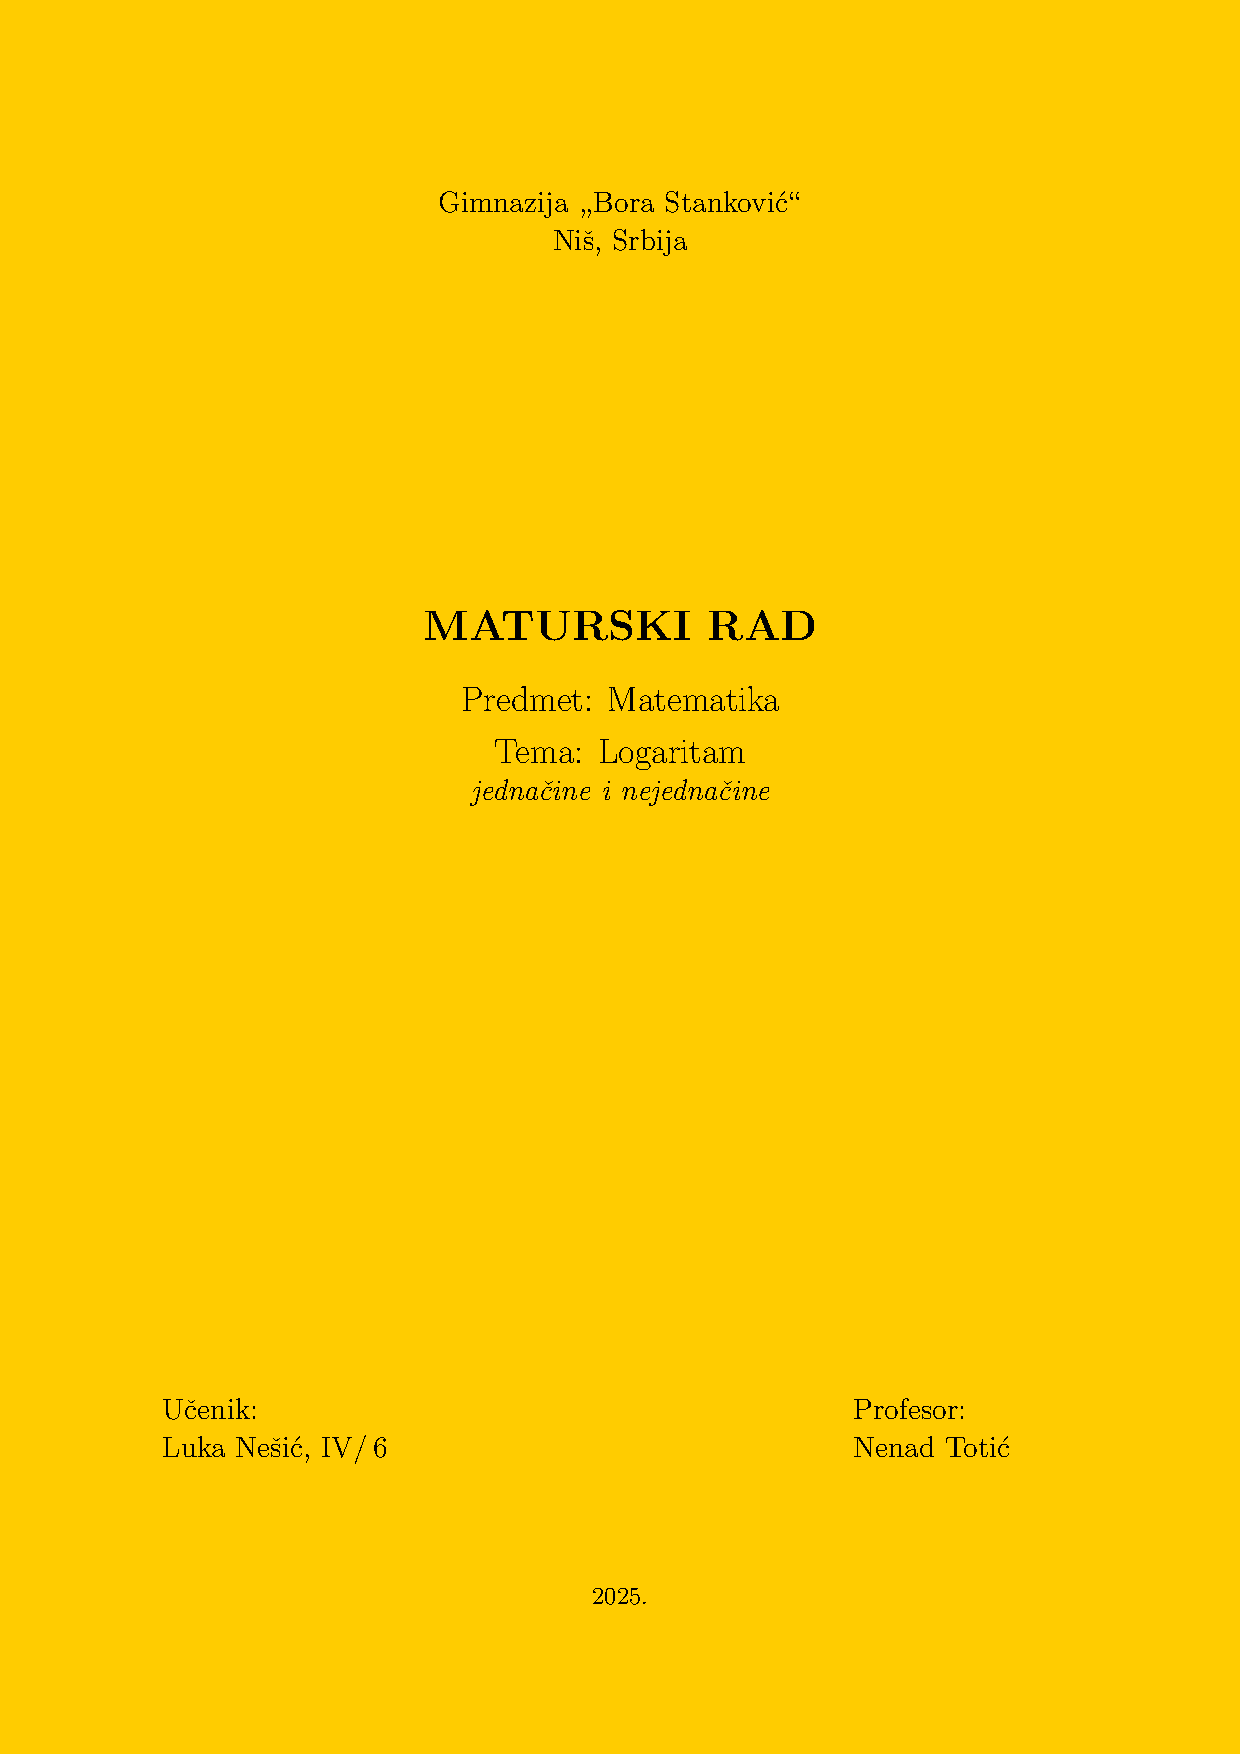
\includegraphics[]{log.2}}{Broj $z$ u kompleksnoj ravni.}
$$
koji mo{\zv}e biti predstav{\lj}ean kao
\begin{alignat*}{3}
z 
&= x + iy &&\qquad\text{pravougle koordinate}\\
&= \rho\, (\cos\theta +i\sin\theta)&&\qquad\text{polarne koordinate}\\
%&= \rho\mathbin{\rm cis}\theta&&\qquad\text{skra{\cc}eni polarni zapis}\\
& = \rho\, \e^{i\theta} &&\qquad\text{Ojlerova formula}
\end{alignat*}
onda se, iz Ojlerove formule i jednakosti \eqref{eq:lnmul} i \eqref{eq:powb}, dobija
\begin{equation}
\okvir{\ln z = \ln\rho + i\theta}.
\label{eq:cln}
\end{equation}
Po{\sv}to je $\rho=|z|=\sqrt{x^2+y^2}\ge0$,
sledi da prirodni logaritam kompleksnog broja $z$ nije definisan ($\rsinfty$) samo za $z=0$.
Kako je $y/x=\tan\theta$, prirodni logaritam kompleksnog broja,
pred\-stav\-{\lj}e\-nog pravouglim koordinatama, iz formule \eqref{eq:cln},
mo{\zv}e se izra{\cv}unati
\begin{equation}
\okvir{\ln(x+iy)=\frac12\ln(x^2+y^2)+i\arctan\left(\frac yx\right)}.
\label{eq:clncart}
\end{equation}
I za kompleksne brojeve va{\zv}i jednakost promene baze \eqref{eq:chgbase}, tako da za dva kompleksna
broja $z$ i $w$, gde je $z\ne0$, $w\ne0$ i $w\ne1$, sledi
$$
\log_w z=\frac{\ln z}{\ln w},
$$
gde se $\ln z$ i $\ln w$ ra{\cv}unaju pomo{\cc}u formule \eqref{eq:cln}, odnosno, \eqref{eq:clncart}.
Na primer,
$$
\log_{2+i}(3+4i)=2, \qquad \log_i\e=\frac{2}{i\pi}.
$$

\medskip

Iz Ojlerove formule se mo{\zv}e dobiti, kako je nazvana, 
{\sl najlep{\sv}a formula u istoriji ma\-te\-ma\-ti\-ke},
u kojoj je upotreb{\lj}eno 5 najva{\zv}nijih matemati{\cv}kih konstatnti 
($0,1,\pi,\e,i$)
\begin{equation}
  \okvir{\e^{i\pi}+1=0},
  \label{eq:zeuler}
\end{equation}
gde, ako prebacimo 1 na desnu stranu i {\sl logaritmujemo}, dobijamo zanim{\lj}ivu jednakost
$$
\frac{\ln(-1)}{\sqrt{-1}}=\pi.
$$


\subsection{Izvod}

Ako je 
$$
y=\ln x\sledi y'=\frac1x,
$$
odakle se, pomo{\cc}u jednakosti \eqref{eq:chgbase} i jednakosti za izvod slo{\zv}ene funkcije, mo{\zv}e dobiti
\begin{equation}
\okvir{y=\logb(f(x))\sledi y'=\frac{f'(x)}{f(x)\ln b}}.
\label{eq:izvod}
\end{equation}

\def\dx{{\it dx}}
Povr{\sv}ina figure ispod funkcije $y=1/x$ do $x$-ose, u opsegu od 1~do~$x$ iznosi 
$\ln x$.\penalty-1000
Matemati{\cv}ki zapisano: $\int_1^x\dx/x=\ln x$.
$$
\slika{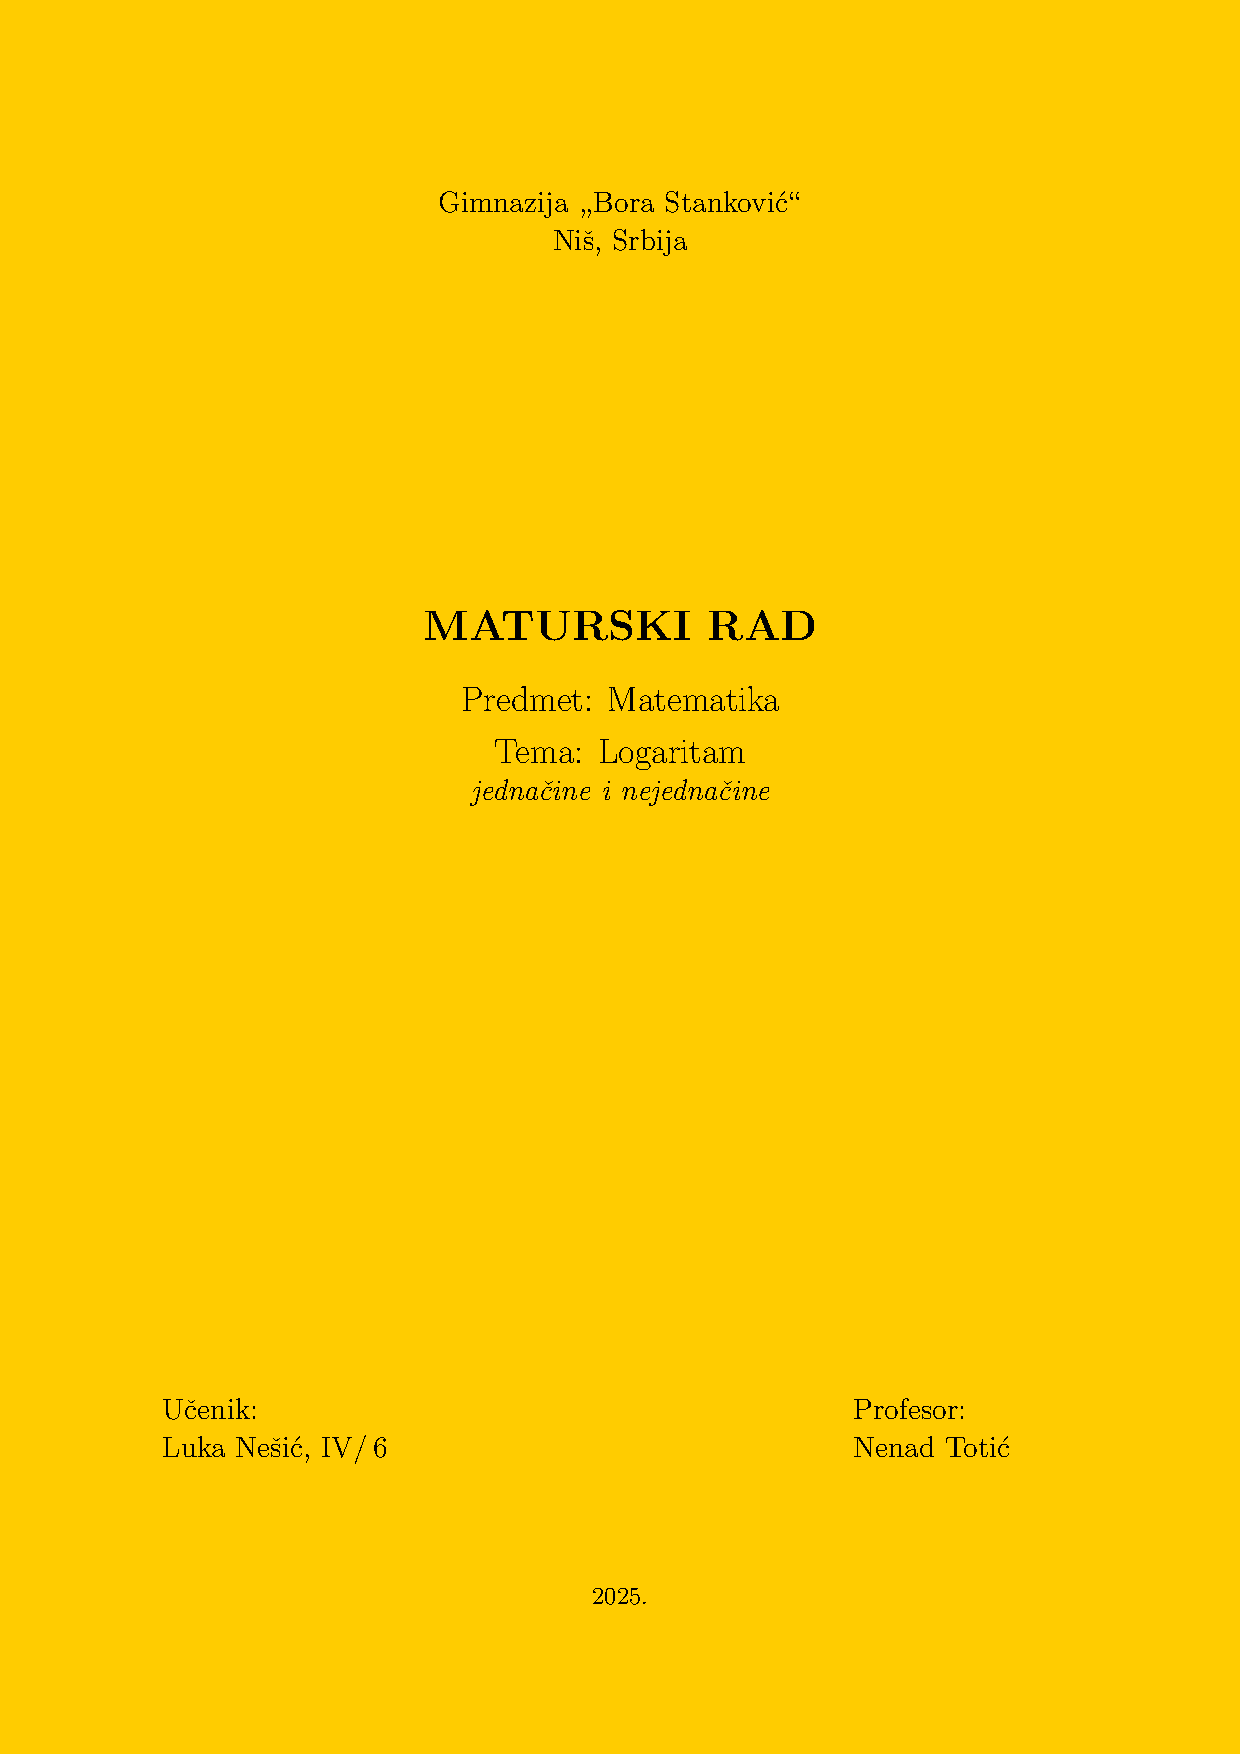
\includegraphics[]{log.3}}{Geometrijsko zna{\cv}e{\nj}e $\ln x$.}
$$
(Na slici je $x=\e$, tako da je povr{\sv}ina osen{\cv}ane figure jednaka 1.)

\medskip

Iz jednskosti $a^x=\e^{x\ln a}$,
mo{\zv}e se dobiti i jednakost
\begin{equation}
  \okvir{f(x)=a^x\sledi f'(x)=a^x \ln a}.
\end{equation}

\subsection{Limes}

Ojler je dokazao da je
$$
\ln x=\lim_{n\to\infty}n(\sqrt[n]x-1).
$$

\subsection{Teorema prostih brojeva}

Jo{\sv} jedno mesto gde se pojav{\lj}uje prirodni logaritam u {\sl teoriji brojeva} je,
takozvana, {\sl teorema prostih brojeva\/} (PNT), kojom se je bavio Gaus kada je
imao samo 15--16 godina.

\smallskip

Ako funkcija $\pi(n)$ ima vrednost {\sl ukupan broj prostih brojeva ma{\nj}ih
ili jednakih od~$n$}, onda va{\zv}i
$$
\lim_{n\to\infty}\frac{\pi(n)\ln n}{n} = 1.
$$
Posledica ove teoreme je da je $n$-ti prost broj $p_n$, za veliko $n$, otprilike
$$
p_n\sim n\ln n.
$$


\section{Zadaci i re{\sv}e{\nj}a}

\subsection{Jedna{\cv}ine}
\def\jed{Jedna{\cv}ina~}

\input zadaci/fit-prijemni
\input zadaci/jed2
\input zadaci/jjjj
\input zadaci/44
\input zadaci/sveska-7
\input zadaci/inf-root
\input zadaci/net3
\input zadaci/log2ser

\clearpage

\subsection{Nejedna{\cv}ine}

\input zadaci/sveska-11
\input zadaci/sveska-9
\input zadaci/sveska-10
%\clearpage
\input zadaci/net1
\input zadaci/net2
\input zadaci/net4
% \input zadaci/net5
\input zadaci/net6

\clearpage

% \addtocontents{toc}{\protect\newpage}

\subsection{Sitni primeri}

\input zadaci/earthquake
\input zadaci/128-bit
\input zadaci/131-I
\input zadaci/geom-serie
\input zadaci/izvod
\input zadaci/i-na-i
\input zadaci/neglog

\clearpage

\subsection{Ru{\cv}ni rad}

\input zadaci/siber-sqrt
\input zadaci/siber-power
\input zadaci/ln3

\vfill

%\rightline{\eightssi \the\exno\ zadataka u ovom radu.}


\section{Reference}

\tolerance=10000

\renewcommand{\labelenumi}{[{\it\arabic{enumi}\/}]}
\def\lit#1#2#3(#4){\item #1: {\navod{#2}}, {\sl#3\/} (#4)}
\font\logoten=logo10 scaled 1200
\def\MP{{\logoten METAPOST}}
\def\link#1#2{\item\href{#1}{#2}\hfill\break\href{#1}{\footnotesize\tt#1}}


\subsection{Linkovi}

\begin{enumerate}[parsep=0cm]
\link{\GitHubRaw log.pdf}{{\sf GitHub} --- Luka S. Ne{\sv}i{\cc} --- Maturski rad --- Logaritam}
\link{https://en.wikipedia.org/wiki/Logarithm}{{\sc WikipediA} --- Logarithm}
\link{https://mathworld.wolfram.com/Logarithm.html}{Wolfram MathWorld --- Logarithm}
\link{https://mathworld.wolfram.com/Antilogarithm.html}{Wolfram MathWorld --- Antiogarithm}
\link{https://reference.wolfram.com/language/ref/Log.html}{Wolfram Language \& System Documentation Center --- Logarithm}
\link{https://www.wolframalpha.com/}{{\sf WolframAlpha} --- Computational Intelligence}
\link{https://inria.hal.science/inria-00543939/PDF/briggs1624doc.pdf}{A reconstruction of the tables of Briggs' {\sl Arithmetica logarithmica\/} (1624)}
\link{https://people.mpim-bonn.mpg.de/zagier/files/doi/10.2307/2975232/fulltext.pdf}{Newman's Short Proof of the Prime Number Theorem}
\link{https://www.youtube.com/watch?v=VRzH4xB0GdM}{{\sf YouTube} --- Log Tables --- Numberphile}
\link{https://www.youtube.com/watch?v=xRpR1rmPbJE}{{\sf YouTube} --- The iPhone of Slide Rules --- Numberphile}
\link{https://www.youtube.com/watch?v=Noo4lN-vSvw}{{\sf YouTube} --- The Four 4s --- Numberphile}
\link{https://github.com/Nasumica/Wirth}{GitHub --- Srbislav D. Ne{\sv}i{\cc} --- Numerical recipes in Pascal}
\end{enumerate}


\subsection{Literatura}

\begin{enumerate}[parsep=0cm]
\lit{Larousse}{Matematika}{Op{\sv}ta enciklopedija}(1967)
\lit{Neboj{\sv}a Ikodinovi{\cc}, Sla{\dj}ana Dimitrijevi{\cc}, Suzana Aleksi{\cc}}{U{\dz}benik sa
zbir\-kom zadataka za 2. razred gimnazije}{Matematika 2}(2019)
\lit{Vene Bogoslavov}{Zbirka re\sv enih zadataka iz matematike 2}{}(2008--2011)
\lit{Marjan M. Mateji\cc, Lidija V. Stefanovi\cc, Branislav M. Ran\dj elovi\cc, Igor \Zv. Milo\-va\-novi\cc}{Kom\-ple\-ti
zadataka za prijemni ispit}{Matematika}(2011)
\lit{Rade Nikoli{\cc}}{Zadaci za prijemni ispit iz matematike na Fakultet informacionih tehnologija}{}(2020)
\lit{Gradimir V. Milovanovi{\cc}, {\Dj}or{\dj}e R. {\Dj}or{\dj}evi{\cc}}{Programira{\nj}e numeri{\cv}kih me\-to\-da}{}(1981)
\lit{Donald E. Knuth}{Seminumerical Algorithms}{The Art of Computer Programming}(1968--)
\lit{Drago{\lj}ub Vasi{\cc}, Vene Bogoslavov, Gli{\sv}a Ne{\sv}kovi{\cc}}{Logaritamske tablice}{}(2008)
\lit{Henry Briggs}{Arithmetica logarithmica}{}(1624)
\lit{Donald E. Knuth}{The \TeX book}{Computers and Typesetting}(1996)
\lit{John D. Hobby}{User's manual}{\MP}(2024)
\end{enumerate}

\subsection{Software}

\newbox\gobox \setbox\gobox\hbox{\textbf{GO}}
\newdimen\godim \godim=\ht\gobox \advance\godim\dp\gobox
\newdimen\down \down=0.03\godim \advance\godim\down
\begin{enumerate}[parsep=0cm]
  \item Mathematica --- Wolfram Research
  \item {\sf Visual Studio Code} (Integrated Development Environment) --- Microsoft
  \item \TeX\ (typesetting system) --- Donald E. Knuth
  \item \LaTeX\ (\TeX\ macros) --- Leslie Lamport
  \item \AmS-\TeX\ (\TeX\ macros) --- American Mathematical Society
  \item \MP\ (PostScript programming language)--- John D. Hobby
  \item \textbf{Pascal} (programming language) --- Niklaus Wirth
  \item \textbf{Python} (programming language) --- Python Software Foundation
  \item \leavevmode\kern-5pt\raise-\down\hbox{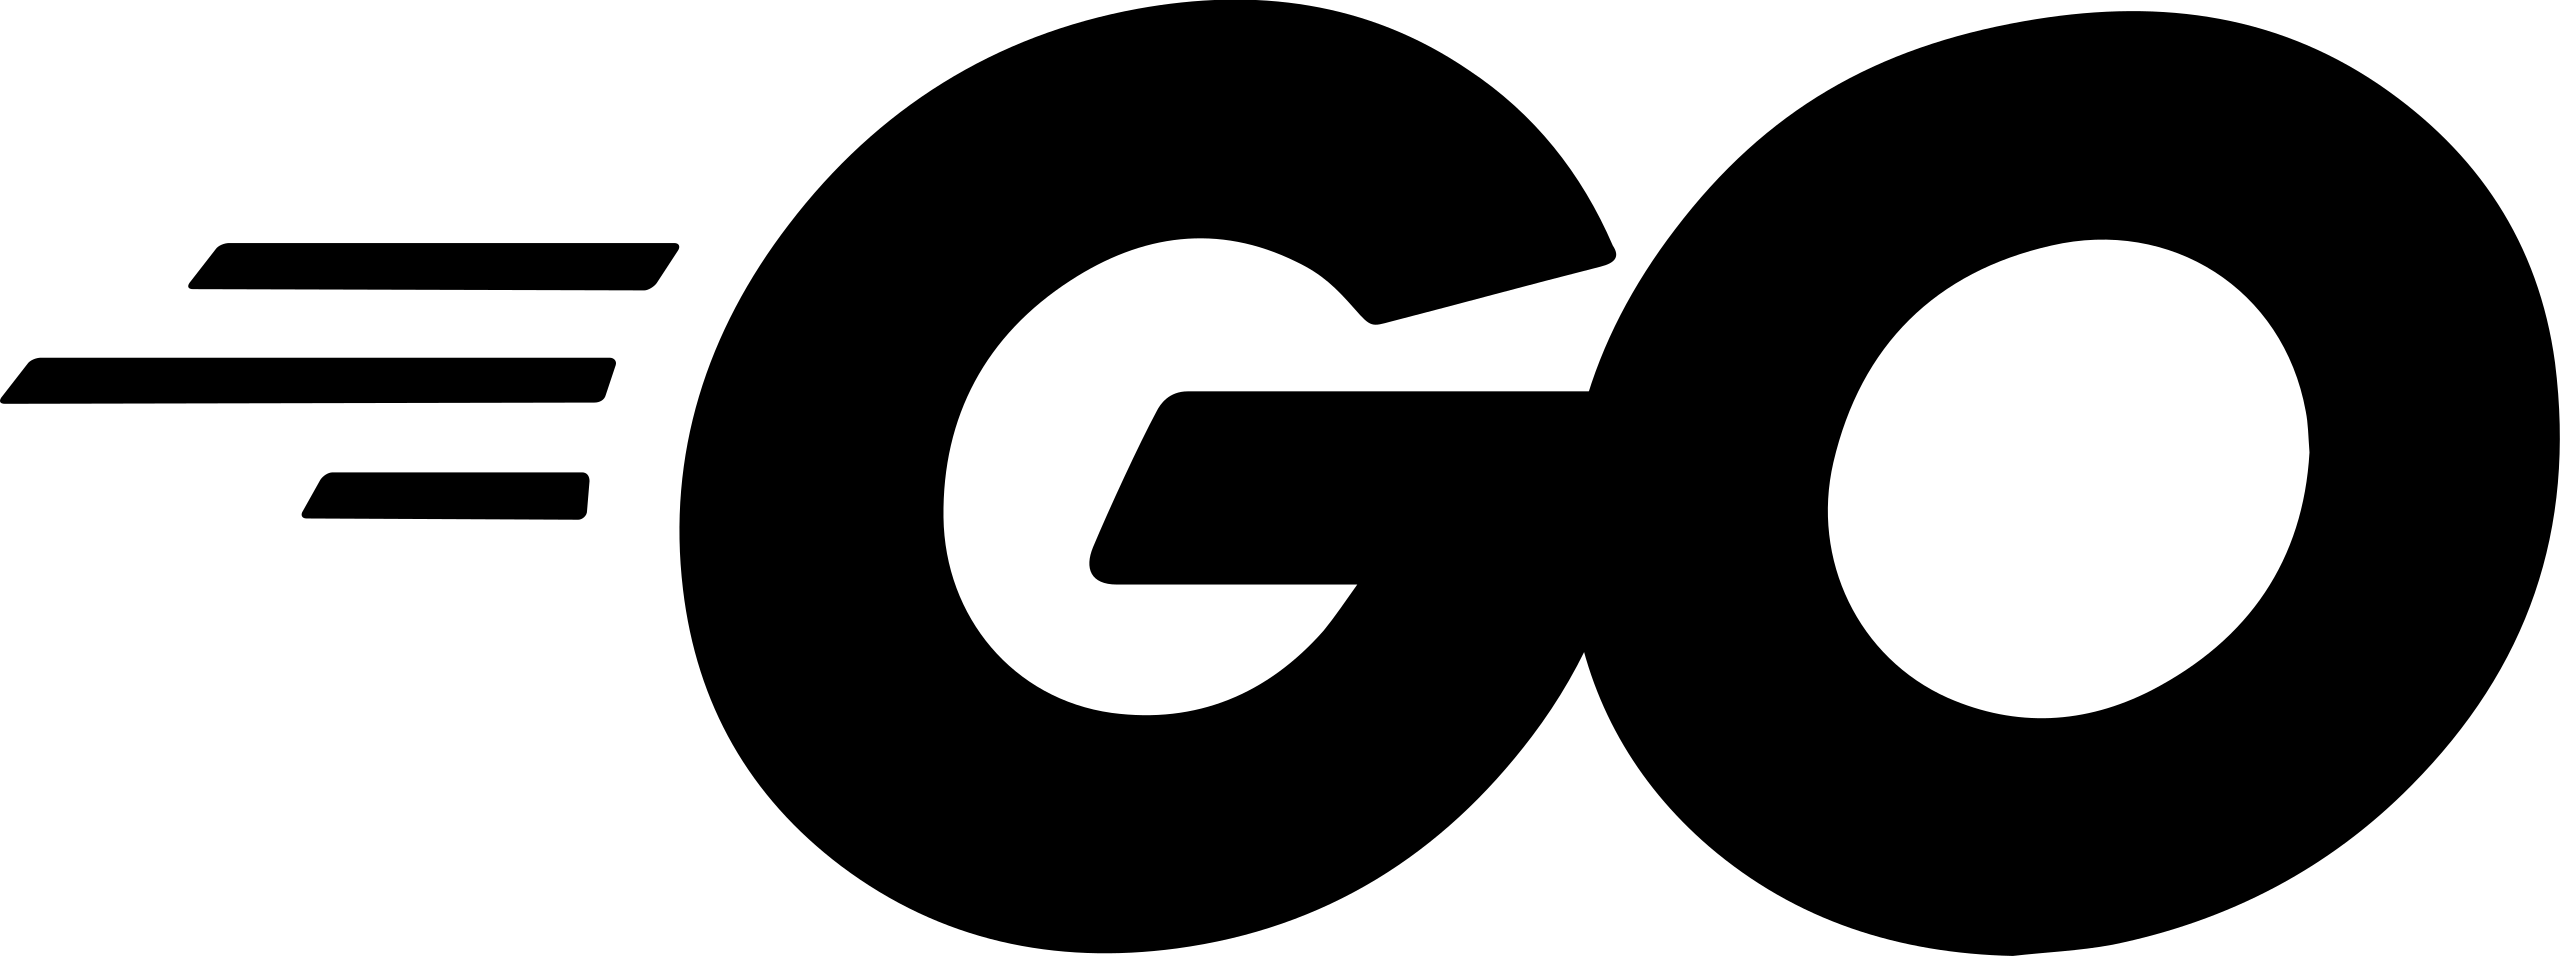
\includegraphics[height=\godim]{GO.png}} (programming language) --- Google
  \item {\ZXBASIC} (programming language) --- Sinclair Research Ltd.
\end{enumerate}


\bigskip

\input dayofweek

\def\twodig#1{\ifnum#1>9\else0\fi\number#1}
\def\datum{\twodig\day.\twodig\month.\number\year.}
\newcount\hour \hour=\time \divide\hour by 60
\newcount\minute \minute=-\hour \multiply\minute by 60
\advance\minute by \time 
\def\vreme{\twodig\hour:\twodig\minute}

% \rightline{\eightssi--- Luka S. Ne{\sv}i{\cc},\enspace\eightss (\the\year)}
\rightline{\eightssi--- \href{mailto:luka.s.nesic@gmail.com}{Luka S. Ne{\sv}i{\cc}},\enspace\eightss\DayOfWeek~\datum~\vreme}

\par\vfill

$$
\slika{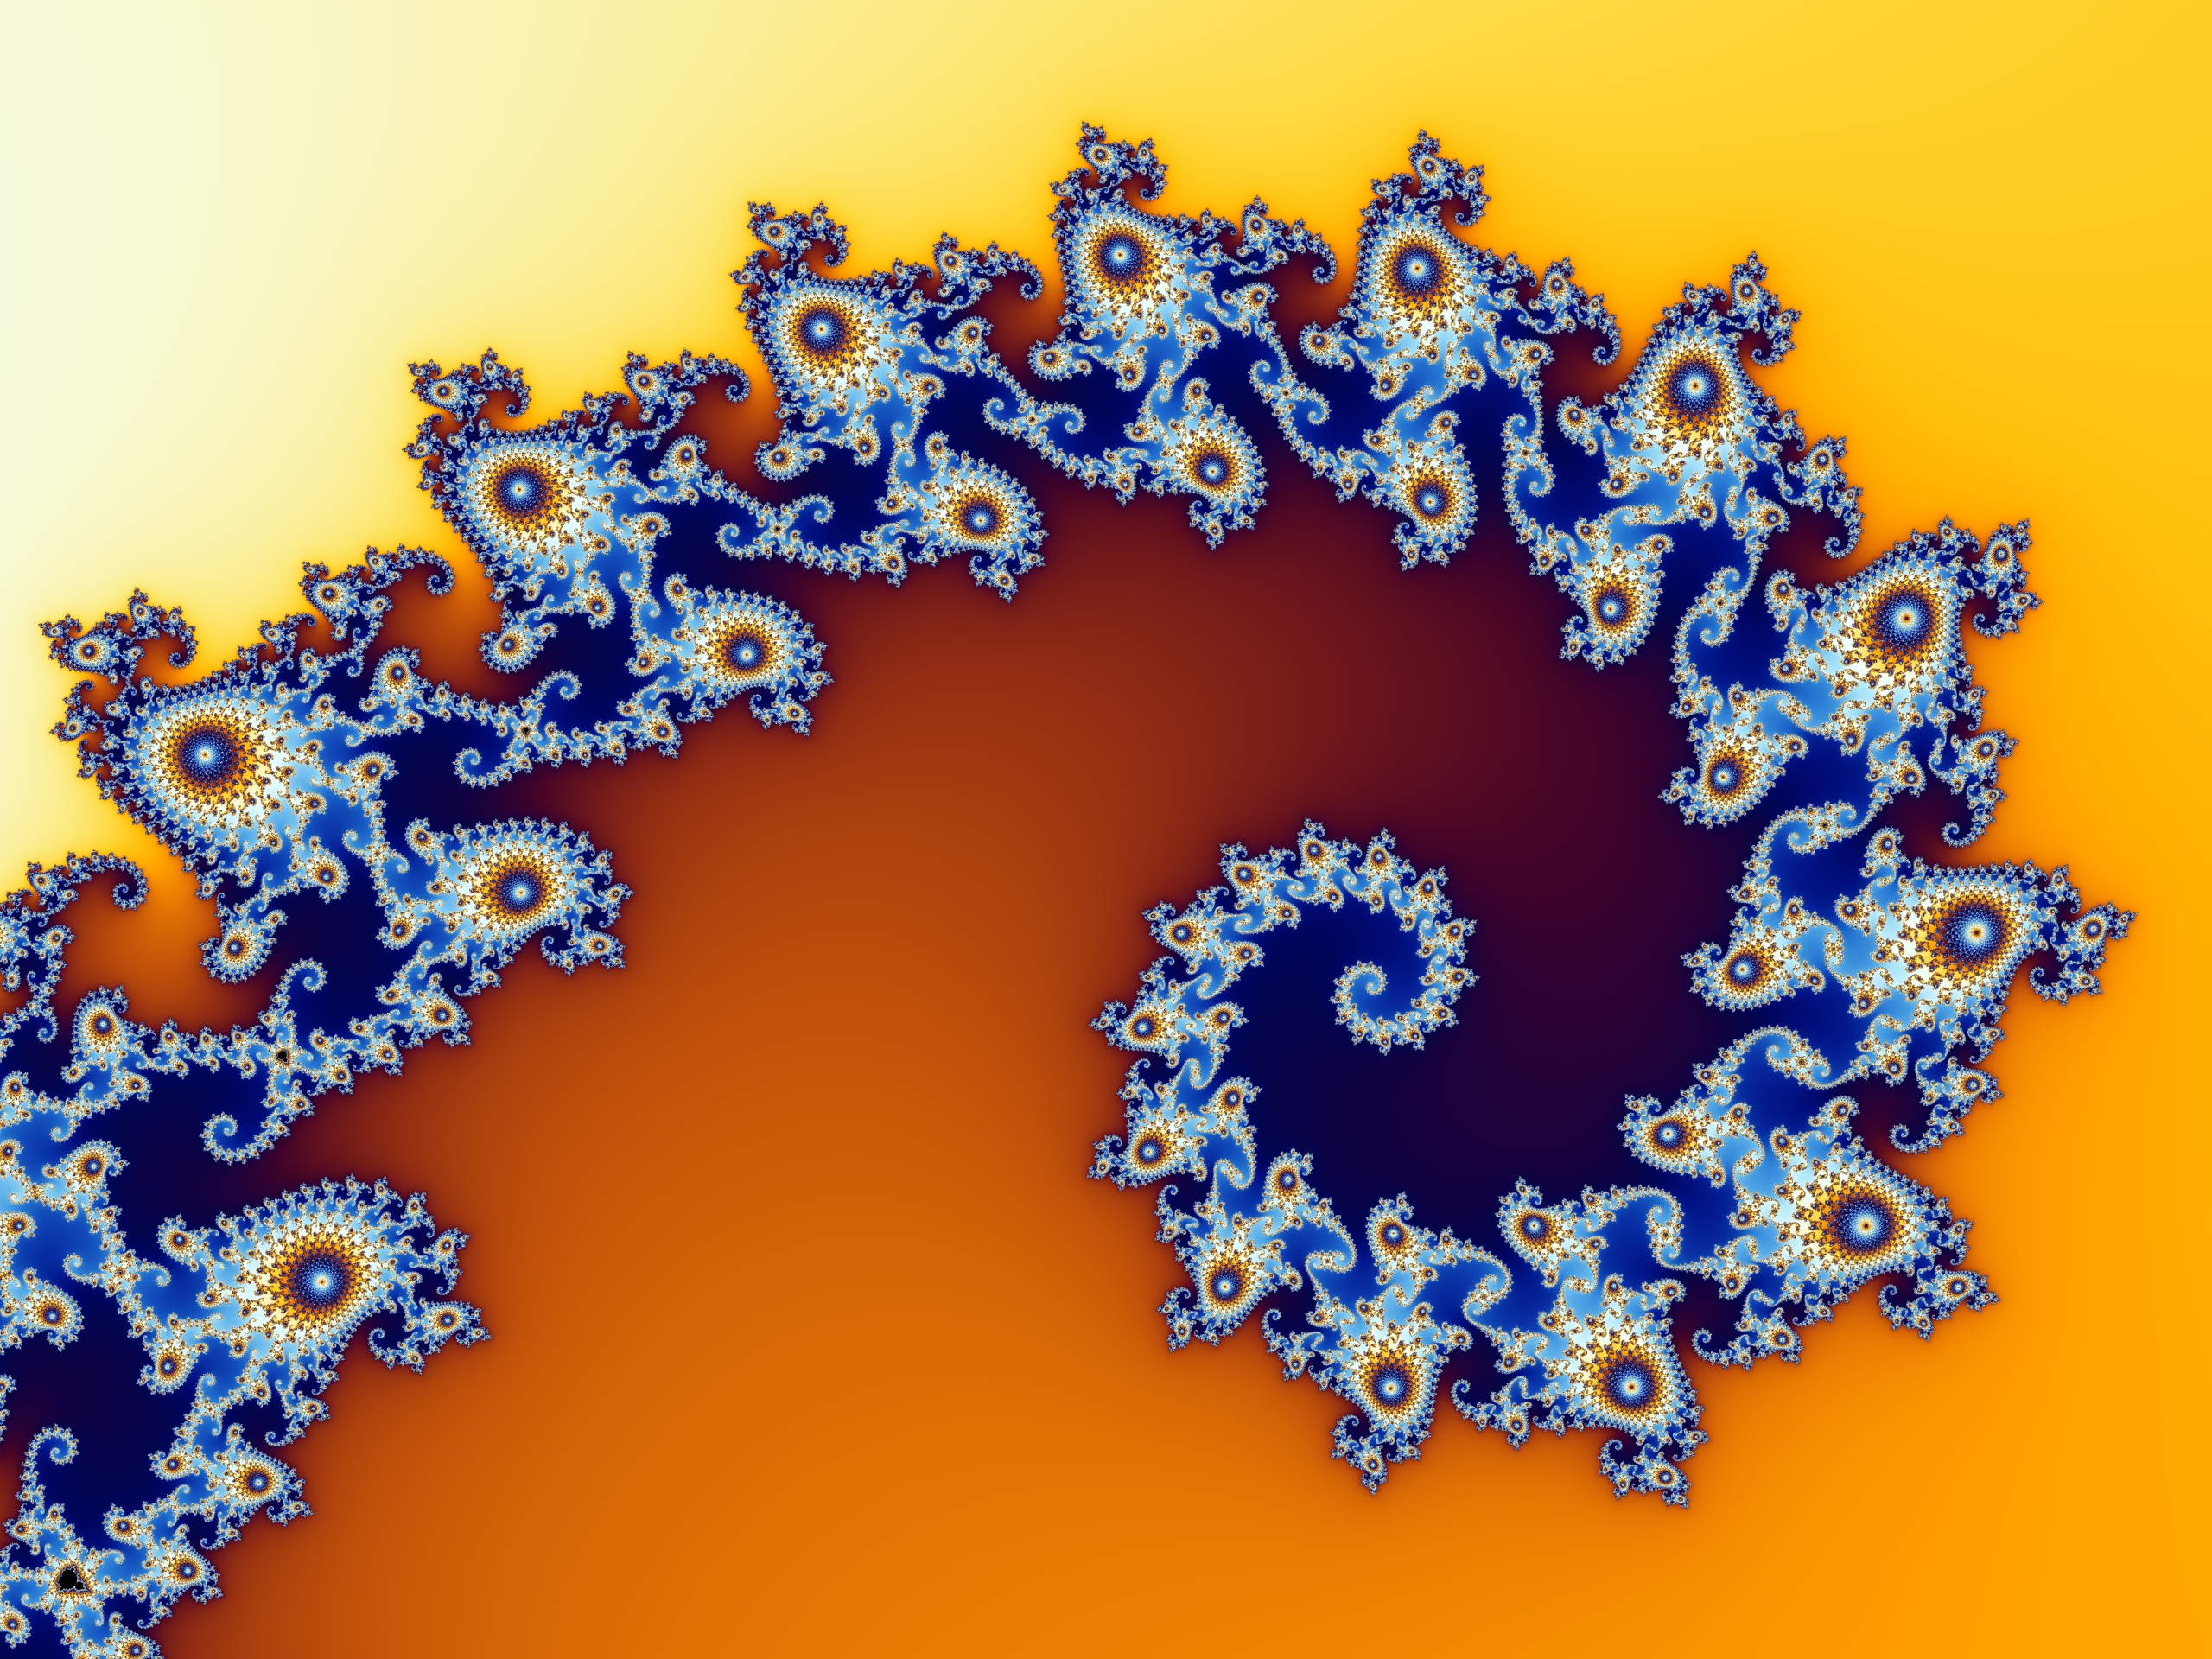
\includegraphics[
  % decodearray={0.5 1 0.5 1 0.5 1},
  width=\textwidth]{mandel-log-spiral.jpg}}{%
\href{https://en.wikipedia.org/wiki/Mandelbrot_set}{Mandelbrotov skup} --- 
\href{https://en.wikipedia.org/wiki/Logarithmic_spiral}{logaritamske spirale}.}
$$

\iffalse
\clearpage

\thispagestyle{empty}
\leavevmode\hbox{}

\vfill

\begin{center}
\qrcode{https://github.com/Nasumica/LukaMaturski/blob/main/log.pdf}
\end{center}
\fi


\end{document}
